\documentclass[a4paper,14pt]{extarticle}
\usepackage[T2A]{fontenc}
\usepackage[utf8]{inputenc}
\usepackage[russian]{babel}

\usepackage[dvips]{graphicx}
\usepackage{color}
\usepackage{hyperref}
%\usepackage{pst-all}

\usepackage{setspace}
\usepackage{indentfirst}
\usepackage{textcomp}
\usepackage{ifthen}
\usepackage{calc}
\usepackage{minted}

%\usepackage[cache=false]{minted}

\hypersetup{%
	unicode,%
	linkcolor=blue,
	colorlinks=true,%
%	pdfpagemode=FullScreen,%
%	pdfpagetransition=Dissolve,%
	pdftitle={Курсовая работа по дисциплине "Операционные системы и архитектура ПК"},%
}


\thispagestyle{empty}

\setlength{\voffset}{-.8in}
\setlength{\hoffset}{-.75in}
\addtolength{\textheight}{1.6in}
\addtolength{\textwidth}{1.5in}


\onehalfspacing

%Поменяйте фамилию, имя и отчество в команде FIO
\newcommand{\FIO}{Грубенко Максим Дмитриевич}

%Поменяйте название программного продукта в команде SOFTWARE
\newcommand{\SOFTWARE}{Частотный анализ встречающихся символов и Калькулятор длинных чисел}

%Укажите номер группы (210 или 211)
\newcommand{\GROUP}{210}

\setcounter{tocdepth}{2}

\begin{document}
\begin{center}
{\large	МИНИСТЕРСТВО НАУКИ И ВЫСШЕГО ОБРАЗОВАНИЯ РФ 
	
	\textbf{Московский авиационный институт }
	
	\textbf{(национальный исследовательский университет)} 
	\bigskip
	
	Институт \textnumero~8 
	
	Информационных технологий и прикладной математики}
	
	\bigskip
	
	\textbf{Кафедра 813 <<Компьютерная математика>>}
	\bigskip
	
	\vfill \textsc{\Large курсовая работа} \\
	{\large по дисциплине <<Операционные системы и архитектура компьютеров>>}
	\bigskip

	на тему: Разработка клиент-серверного программного комплекса
	
	<<\SOFTWARE>>
\end{center}
\vspace*{1.5cm}

\hfill 
\begin{minipage}{.6\linewidth}\
\begin{tabular}{c}
\textbf{Выполнил:} студент группы М8О-\GROUP{}Б-20 \\\hline \\[.3cm]
{\large \FIO} \\ \hline \scriptsize{(Фамилия, имя, отчество)}
\\[.3cm] \\ \hline
\scriptsize{(подпись)} \\[.3cm]
\textbf{Принял: }\hfill профессор кафедры 813 \\\hline 
\\[.3cm]

Чернова Татьяна Александровна\\\hline 
\scriptsize{(Фамилия, имя, отчество)}
\\[.3cm] \\ \hline
\scriptsize{(подпись)} 
\end{tabular}
\vspace*{1cm}
\end{minipage}		

\centerline{\textbf{Оценка}: \hspace*{8cm} \textbf{Дата}: \hspace*{2cm}}
\vspace*{1cm}

\centerline{Москва, 2021}

\newpage

\tableofcontents
\newpage
\
\part{Общая часть}
\section{Работа с процессами}
\subsection{Используемые системные объекты}
Процесс --- это идентифицируемая абстракция совокупности взаимосвязанных системных ресурсов на основе отдельного и независимого виртуального адресного пространства в контексте которой организуется выполнение потоков. В операционной системе процессы представляются определенной
структурой данных, отражающей содержание регистрового и системного контекстов.
Обычно процесс в вычислительной системе представлен следующими ресурсами:
\begin{itemize}
	\item образом исполняемого машинного кода, ассоциированного с программой;
	\item памятью (обычно некоторой областью виртуальной памяти), которая включает в себя:
	исполняемый код;
	\item входные и выходные данные процесса;
	\item стек вызовов (для отслеживания активных подпрограмм);
	\item кучу для хранения промежуточных результатов вычислений, генерируемых во время выполнения;
	\item дескрипторами ресурсов операционной системы, выделенными для процесса, например, файл
	файловыми дескрипторами (в терминологии ОС Unix) или «хэндлами» (в терминологии ОС Windows);
	\item атрибутами безопасности, такими как владелец и набор полномочий процесса (допустимых операций);
	\item состоянием процессора (контекстом), таким как:
	\begin{itemize}
		\item содержимое регистров;
		\item схема преобразования виртуальных адресов в физические;
		\item и т. д.
	\end{itemize}	
\end{itemize}

Контекст текущего процесса выгружается в память, когда выполняется переключение на другой процесс. Операционная система хранит большую часть информации о процессах в таблице процессов.

Каждый процесс в Unix имеет уникальный числовой идентификатор PID. Процессы в ней имеют древовидную иерархию, где корнем является процесс \verb|init| c PID 1. Новый процесс можно создать системным вызовом \verb|fork|, он будет являться точной копией процесса родителя. Любой процесс кроме \verb|init| всегда имеет процесс родитель (атрибут PPID (англ. Parent PID)); процессы, родитель которых завершил свою работу становятся дочерними процессами \verb|init|.

\verb|pid_t fork(void);|

Системный вызов \verb|fork| создает процесс-потомок, который отличается от родительского только значениями PID (идентификатор процесса) и PPID (идентификатор родительского процесса), а также тем фактом, что счетчики использования ресурсов установлены в 0. Блокировки файлов и сигналы, ожидающие обработки, не наследуются.
\subsection{Порождение процессов}
\subsubsection{Техническое задание}
Написать программный комплекс, который состоит из двух частей:

a.	Первая получает на вход (через командную строку) арифметический пример (вещественные числа со знаком и операции: $+$, $-$, $*$, $/$), решает его и печатает ответ.

b.	Написать программу, которая через командную строку принимает текстовый файл со строчками-арифметическими примерами (см. пункт а). Необходимо для каждой прочитанной строки создавать новый процесс, который запускает первую программу с аргументом - прочитанной строкой. Результат работы программы вместе с примером печатается в выходной файл, имя которого передаётся также через аргументы командной строки второй программы.

\subsubsection{Описание основного алгоритма}
Программа через аргументы командной строки принимает пути к двум файлам: файл с арифметическими выражениями и файл для предоставление решения. Файл читается построчно и для каждой через \verb|execl()| запускает программу-калькулятор, которая проводит вычисления и записывает ответ во второй файл.

Реализация алгоритмов представлена в разделе приложения \ref{code:lab1_1}.

\subsubsection{Руководство пользователя}

При запуске необходимо передать в качестве аргументов командной строки имя файла с задачей и имя файла, в который будет записан ответ.

\begin{figure}[h]
\center{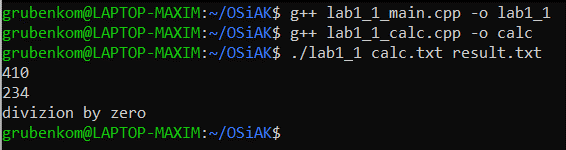
\includegraphics{1.1.png}}
\caption{Компиляция и запуск приложения.}
\label{1.png}
\end{figure}

\begin{figure}[h]
\center{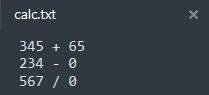
\includegraphics{1.2.png}}
\caption{Задача из файла calc.txt.}
\label{1.png}
\end{figure}

\begin{figure}[h]
\center{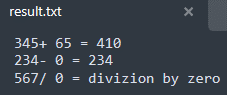
\includegraphics{1.3.png}}
\caption{Решение задачи в файле result.txt.}
\label{1.png}
\end{figure}

\subsection{Ветвящиеся процессы}
\subsubsection{Техническое задание}
Написать программу генерирующие ветвящиеся процессы, по следующему правилу: каждый процесс единожды определяет случайное событие ---
\begin{itemize}
	\item 25\% вероятность завершения процесса; 
	\item 40\% вероятность порождения 1 процесса; 
	\item 25\% вероятность порождения 2 процессов; 
	\item 10\% вероятность порождения 3 процессов.
\end{itemize} 

Нарисуйте гистограмму распределения длин цепочек порождённых процессов, у которых выпало событие завершения процесса. 

Примечание: после выбора любого варианта процесс ждёт завершения всех порождённых процессов и только тогда завершается. 

\subsubsection{Описание основного алгоритма}
С помощью функции \verb|generate_random()|, которая извлекает энтропию из источника \verb|urandom (/dev/urandom)| определяется количество процессов которое необходимо сгенерировать. Далее функция \verb|generate_process()| генерирует необходимое число процессов и количество процессов с n-количеством родителей записывает в файл. В главной функции этот файл обрабатывается и выводится гистограмма распределения длин  цепочек порожденных процессов.

Реализация алгоритмов представлена в разделе приложения \ref{code:lab1_2}.

\subsubsection{Руководство пользователя}
Необходимо запустить программу без аргументов и дождаться отрисовки гистограммы.

\begin{figure}[h]
\center{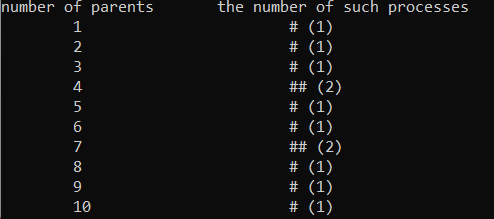
\includegraphics{1_2.1.png}}
\caption{Число родителей и количество этих процессов.}
\label{1.png}
\end{figure}
\newpage

\section{Работа с файловой системой}
\subsection{Используемые системные объекты}
Структура \verb|dirent| в основном предназначена для определения типа файла, но также предоставляет данные о имени файла, индексном дескрипторе и т.д.
\begin{verbatim}
struct dirent {
    ino_t          d_ino;       inode number
    off_t          d_off;       offset to the next dirent
    unsigned short d_reclen;    length of this record
    unsigned char  d_type;      type of file;
    char           d_name[256]; filename
};
\end{verbatim}

Структура \verb|stat| предоставляет доступ к информации о файле. Можно узнать о всех атрибутах файла, таких как режим доступа, количество жестких ссылок, время посленего доступа, последней модификации и т.д.

\begin{verbatim}
struct stat {
    dev_t         st_dev;      /* устройство */
    ino_t         st_ino;      /* inode */
    mode_t        st_mode;     /* режим доступа */
    nlink_t       st_nlink;    /* количество жестких ссылок */
    uid_t         st_uid;      /* идентификатор пользователя-владельца */
    gid_t         st_gid;      /* идентификатор группы-владельца */
    dev_t         st_rdev;     /* тип устройства (если это устройство) 
    off_t         st_size;     /* общий размер в байтах */
    blksize_t     st_blksize;  /* размер блока ввода-вывода */
    blkcnt_t      st_blocks;   /* количество выделенных блоков */
    time_t        st_atime;    /* время последнего доступа */
    time_t        st_mtime;    /* время последней модификации */
    time_t        st_ctime;    /* время последнего изменения */
};
\end{verbatim}

Mакрос \verb|__FILE__| содержит расположение файла исходного кода.

Функция \verb|symlink()| создает символическую ссылку.
Эта ссылка может указывать как на существующий файл, так и на несуществующий.

Функция \verb|link()| создает новую ссылку (также известную как жесткая ссылка) на существующий файл.

\subsection{Реализация ls}
\subsubsection{Техническое задание}
Вывести на экран все файлы, расположенные в директории, введённой пользователем.

\subsubsection{Описание основного алгоритма}
Открываем директорию, имя которой пользователь вводит в программе, с помощью \verb|opendir()| и с помощью \verb|readdir()| получаем указатель на структуру \verb|struct dirent|. В структуре содержится имя файла, которое выводится пользователю.

Реализация алгоритмов представлена в разделе приложения \ref{code:lab2_1}.

\subsubsection{Руководство пользователя}
Необходимо ввести путь к необходимой директории. Программа выведет все файлы и папки, расположенные в ней.

\begin{figure}[h]
\center{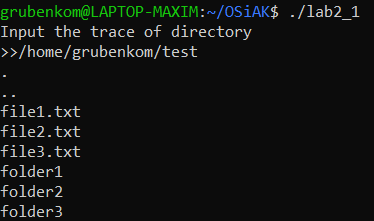
\includegraphics{2_1.png}}
\caption{Результат работы программы.}
\label{1.png}
\end{figure}

\subsection{Реализация ls без папок}
\subsubsection{Техническое задание}
Вывести на экран из указанной пользователем директории все файлы, не являющиеся папками.

\subsubsection{Описание основного алгоритма}
Открываем директорию, имя которой пользователь вводит в программе, с помощью \verb|opendir()| и с помощью \verb|readdir()| получаем указатель на структуру \verb|struct dirent|. В структуре содержится тип файла. Пока он не равен \verb|DT_DIR| выводим пользователю название файла, который не является папкой.

Реализация алгоритмов представлена в разделе приложения \ref{code:lab2_2}.

\subsubsection{Руководство пользователя}
Необходимо ввести путь к необходимой директории. Программа выведет все файлы, исключая папки, расположенные в ней.

\begin{figure}[h]
\center{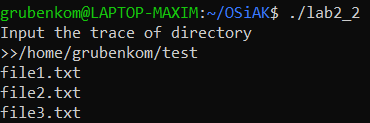
\includegraphics{2_2.png}}
\caption{Программа распечатала имена всех файлов, которые не являются папками.}
\label{1.png}
\end{figure}

\subsection{Жёсткая ссылка}
\subsubsection{Техническое задание}
Открыть указанный файл на запись. Если файл уже существует, сделать на него жёсткую ссылку (\textbf{\texttt{name.x.ext}}), где \textbf{\texttt{x}} --- первый свободный номер, \textbf{\texttt{ext}} --- текущее расширение файла.

\subsubsection{Описание основного алгоритма}
Функция формирует название для жесткой ссылки по заданному шаблону и с помощью функции \verb|link()| создает жесткую ссылку.

Реализация алгоритмов представлена в разделе приложения \ref{code:lab2_3}.

\subsubsection{Руководство пользователя}
Необходимо ввести имя файла, которому нужно создать ссылку. Программа в результате создаст ссылку и выведет ее название пользователю.

\begin{figure}[h]
\center{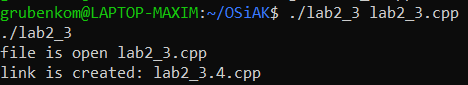
\includegraphics{2_3.png}}
\caption{Создана жесткая ссылка на файл с исходным кодом программы.}
\label{1.png}
\end{figure}

\subsection{Символическая ссылка}
\subsubsection{Техническое задание}
Создать символическую ссылку на файл с текстом программы по указанному пути и вывести информацию по ней об атрибутах данной символической ссылки.

\subsubsection{Описание основного алгоритма}
Программа создает символическую ссылку посредством функции \verb|symlink()| на файл с исходным кодом программы и с помощью структуры \verb|struct stat| выводит информацию об атрибутах созданной ссылки.

Реализация алгоритмов представлена в разделе приложения \ref{code:lab2_4}.

\subsubsection{Руководство пользователя}

Необходимо передать через аргументы командной строки имя файла, которому требуется создать символическую ссылку и дождаться завершения работы программы.

\begin{figure}[h]
\center{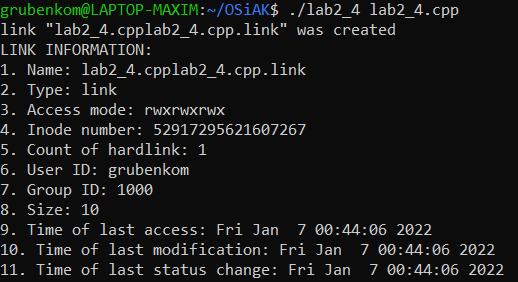
\includegraphics{2_4.png}}
\caption{Демонстрация создания символической ссылки и вывод в консоль ее атрибутов.}
\label{1.png}
\end{figure}

\subsection{Сортировка файлов}
\subsubsection{Техническое задание}
Вывести на экран информацию обо всех файлах в директории, отсортированную по времени последнего изменения файла.

\subsubsection{Описание основного алгоритма}
Программа, читая переданную пользователем директорию, заносит информацию о файле в вектор пар, которая содержит поля имя файла и дата последнего изменения. С помощью функции \verb|sort()|, которая определена в \verb|algorithm|, сортируется созданный вектор и выводится в консоль пользователю.

Реализация алгоритмов представлена в разделе приложения \ref{code:lab2_5}.

\subsubsection{Руководство пользователя}
Требуется в программе написать путь к директории, содержимое которой надо вывести в отсортированном, по дате последнего изменения, виде.

\begin{figure}[h]
\center{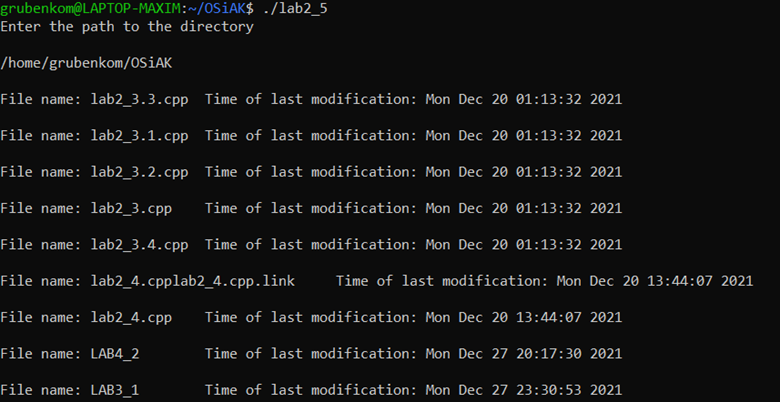
\includegraphics{2_5.png}}
\caption{Файлы заданной директории выводятся в консоль в отсортированном виде.}
\label{1.png}
\end{figure}

\newpage

\section{Локальная клиент-серверная модель}
\subsection{Используемые системные объекты}
\subsubsection{Очередь сообщений}
Очередь сообщений — это связный список, находящийся в адресном пространстве ядра. Каждая очередь имеет свой уникальный идентификатор IPC.

\begin{verbatim}
#include <types.h>
#include <ipc.h>
#include <msg.h>

int msgget(key_t key, int msgflg);
\end{verbatim}

Для создания очереди сообщений, ассоциированной с определенным ключом, или доступа по ключу к уже существующей очереди используется системный вызов \verb|msgget()|, который возвращает значение IPC-дескриптора для этой очереди. Дескриптор System V IPC --- целое неотрицательное число, однозначно характеризующее очередь сообщений внутри вычислительной системы и использующееся в дальнейшем для других операций с ней.

Параметр \verb|key| является ключом System V IPC для очереди сообщений, т. е. фактически ее именем из пространства имен System V IPC. В качестве значения этого параметра может быть использовано значение ключа, полученное с помощью функции \verb|ftok()|, или специальное значение \verb|IPC_PRIVATE|. Использование значения \verb|IPC_PRIVATE| всегда приводит к попытке создания новой очереди сообщений с ключом, который не совпадает со значением ключа ни одной из уже существующих очередей и не может быть получен с помощью функции \verb|ftok()| ни при одной комбинации ее параметров.
\begin{verbatim}
    int msgsnd(int msqid, struct msgbuf *ptr, int length, int flag);
\end{verbatim}

Системный вызов \verb|msgsnd()| предназначен для помещения сообщения в очередь сообщений.

Параметр \verb|msqid| является дескриптором System V IPC для очереди, в которую отправляется сообщение, т. е. значением, которое вернул системный вызов \verb|msgget()| при создании очереди или при ее поиске по ключу.

Структура \verb|struct msgbuf| описана в файле \verb|<sys/msg.h>| как:
\begin{verbatim}
struct msgbuf {
    long mtype;
    char mtext[1];
};
\end{verbatim}
Она представляет собой некоторый шаблон структуры сообщения пользователя. Сообщение пользователя --- это структура, первый элемент которой обязательно имеет тип \verb|long| и содержит тип сообщения, а далее следует информативная часть (в Linux длина ограничена 4080 байт).

\begin{verbatim}
int msgrcv(int msqid, struct msgbuf *ptr,int length, long type, int flag);
\end{verbatim}

Системный вызов \verb|msgrcv()| предназначен для получения сообщения из очереди сообщений. 

Параметр \verb|type| определяет способ выборки сообщения из очереди.

\begin{verbatim}
int msgctl(int msqid, int cmd, struct msqid_ds *buf);
\end{verbatim}

Системный вызов \verb|msgctl()| предназначен для получения информации об очереди сообщений, изменения ее атрибутов и удаления из системы.

Для удаления очереди в качестве параметра \verb|cmd| необходимо передавать значение \verb|IPC_RMID|. Параметр \verb|buf| для этой команды не используется, поэтому подставляется туда значение \verb|NULL|.

\subsubsection{Семафоры}

Семафор --- примитив синхронизации работы процессов и потоков, в основе которого лежит счётчик, над которым можно производить две атомарные операции: увеличение и уменьшение значения на единицу, при этом операция уменьшения для нулевого значения счётчика является блокирующей.

\begin{verbatim}
#include <sys/types.h>
#include <sys/ipc.h>
#include <sys/sem.h>

int semget(key_t key, int nsems, int semflg);
\end{verbatim}

Системный вызов \verb|semget()| предназначен для выполнения операции доступа к массиву IPC-семафоров и, в случае ее успешного завершения, возвращает дескриптор System V IPC для этого массива.

Параметр \verb|key| является ключом System V IPC для массива семафоров, т. е. фактически его именем из пространства имен System V IPC. В качестве значения этого параметра может использоваться значение ключа, полученное с помощью функции \verb|ftok()|.

Параметр \verb|nsems| определяет количество семафоров в создаваемом или уже существующем массиве.

\begin{verbatim}
int semop(int semid, struct sembuf *sops, int nsops);
\end{verbatim}

Системный вызов производит операции над выбранными элементами из набора семафоров \verb|semid|. Каждый из элементов \verb|nsops| в массиве \verb|sops| определяет операцию, производимую над семафором в структуре \verb|struct sembuf|.

\begin{verbatim}
struct sembuf {
    short sem_num;
    short sem_op;
    short sem_flg;
};
\end{verbatim}

Флаги в \verb|sem_flg| могут иметь значения \verb|IPC_NOWAIT| и \verb|SEM_UNDO|. Если стоит флаг \verb|SEM_UNDO|, то будет выполнена обратная операция при закрытии процесса.
\begin{verbatim}
int semctl(int semid, int semnum, int cmd, union semun arg);
\end{verbatim}

Системный вызов \verb|semctl| предназначен для получения информации о массиве IPC семафоров, изменения его атрибутов и удаления его из системы.

\subsubsection{Разделяемая память}

Разделяемая память является самым быстрым средством обмена данными между процессами.

Техника разделяемой памяти позволяет осуществлять обмен информацией через общий для процессов сегмент памяти без использования системных вызовов ядра. Сегмент разделяемой памяти подключается в свободную часть виртуального адресного пространства процесса. Таким образом, два разных процесса могут иметь разные адреса одной и той же ячейки подключенной разделяемой памяти.

\begin{verbatim}
#include <sys/types.h>
#include <sys/ipc.h>
#include <sys/shm.h>

int shmget(key_t key, int size, int shmflg);
\end{verbatim}

Системный вызов shmget предназначен для выполнения операции доступа к сегменту разделяемой памяти и, в случае его успешного завершения, возвращает дескриптор System V IPC для этого сегмента.

При совместном использовании флага \verb|IPC_CREAT| и \verb|IPC_EXCL| и существовании сегмента с указанным ключом, доступ к сегменту не производится и констатируется ошибочная ситуация, при этом переменная \verb|errno|, примет значение \verb|EEXIST|.

\begin{verbatim}
    char *shmat(int shmid, char *shmaddr, int shmflg);
\end{verbatim}

Системный вызов \verb|shmat()| предназначен для включения области разделяемой памяти в адресное пространство текущего процесса.

Параметр \verb|shmid| является дескриптором System V IPC для сегмента разделяемой памяти, т. е. значением, которое вернул системный вызов \verb|shmget()| при создании сегмента или при его поиске по ключу.

\begin{verbatim}
int shmdt(char *shmaddr);
\end{verbatim}

Системный вызов \verb|shmdt()| предназначен для исключения области разделяемой памяти из адресного пространства текущего процесса.

Параметр \verb|shmaddr| является адресом сегмента разделяемой памяти,т. е. значением, которое вернул системный вызов \verb|shmat()|.

\begin{verbatim}
int shmctl(int shmid, int cmd, struct shmid_ds *buf);
\end{verbatim}

Системный вызов \verb|shmctl()| позволяет пользователю получать информацию о разделяемых сегментах памяти, устанавливать владельца, группу разделяемого сегмента, права на него. Эта функция может также удалить сегмент при условии передачи в параметр \verb|cmd| команды \verb|IPC_RMID|.

\subsection{Очередь сообщений}
\subsubsection{Техническое задание}
С помощью очереди сообщений организовать клиент-серверную модель для решения кубического уравнения. ПО должно делать следующее 
\begin{enumerate}
	\item Пользователь в клиенте задаёт 4 коэффициента и посылает их серверу в одном сообщении вместе со своим PID.
	\item Сервер принимает сообщение и посылает три корня клиенту.
	\item Клиентов может быть много. Каждый из них ждёт сообщение с типом равным своему PID.
\end{enumerate}

\subsubsection{Описание основного алгоритма}
Сервер создает очередь сообщений, к которой подключаются клиенты. В бесконечном цикле сервер читает очередь и при условии, что там появляется сообщение, вычитывает его, получая коэффициенты для кубического уравнения. Коэффициенты передаются в функцию для нахождения корней, которая записывает результат вычислений в структуру. Затем сервер отправляет полученные данные в очередь, откуда клиент вычитывает данные и выводит их пользователю в консоль.

Реализация алгоритмов представлена в разделе приложения \ref{code:lab3_1}.

\subsubsection{Руководство пользователя}
Необходимо ввести 4 коэффициента кубического уравнения через пробел и ожидать результата.

\begin{figure}[h]
\center{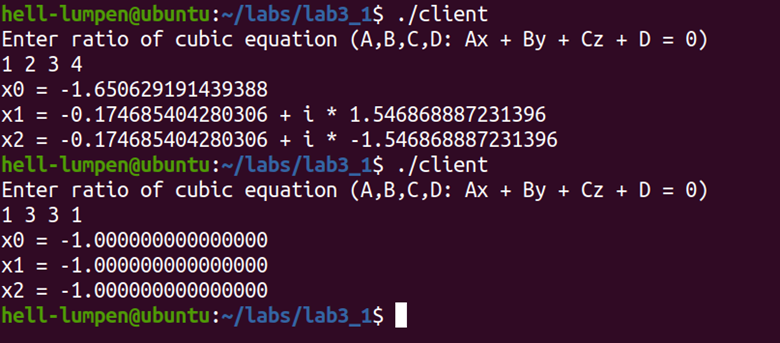
\includegraphics{3_1.png}}
\caption{В левом терминале запущен сервер, а в правом --- клиент.}
\label{1.png}
\end{figure}

\newpage

\subsection{Семафоры и разделяемая память}
\subsubsection{Техническое задание}
Реализовать клиент-сервер на семафорах и разделяемой памяти. Он должен делать следующее: 
\begin{enumerate}
	\item сервер принимает от клиента запросы в виде примера из двух вещественных чисел и бинарной операции между ними ($+$, $*$, $-$, $/$);
	\item сервер возвращает ответ;
	\item клиентов может быть много;
	\item запросы клиенты отправляют в интерактивном режиме;
	\item клиент завершается, если пользователь напечатает пустую строку.
\end{enumerate}

\subsubsection{Описание основного алгоритма}
Инициируются массивы семафоров, которые будут управлять доступом к разделяемой памяти. Сервер открывает сегмент разделяемой памяти и блокируется до того момента, как клиент положит сообщение в открытый сегмент. После этого клиент разблокирует сервер. Он прочитает сообщение, решит пример и положит в память ответ и заблокируется, открыв доступ к памяти для клиента, который, в свою очередь прочитает ответ клиента и выведет его пользователю в терминал. 

Реализация алгоритмов представлена в разделе приложения \ref{code:lab3_2}.

\subsubsection{Руководство пользователя}
Для решения примера необходимо написать выражение, разделяя числа и знак пробелом. Клиент работает в интерактивном режиме, поэтому можно множество раз отправлять запрос с выражением к серверу для решения примера.
\begin{figure}[h]
\center{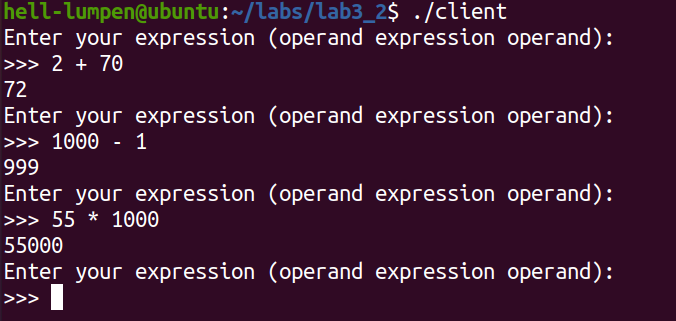
\includegraphics{3_2.png}}
\caption{Клиент работает в интерактивном режиме, ожидая запрос пользователя.}
\label{1.png}
\end{figure}
\newpage

\section{Сетевое программирование}
\subsection{Используемые системные объекты}
TCP является протоколом транспортного уровня. Он позволяет осуществить соединение одного сокета (IP-адрес + порт) хоста источника с сокетом хоста назначения. Заголовок IP будет содержать информацию, связанную с IP-адресами, а заголовок TCP — информацию о порте.

UDP --- протокол транспортного уровня пользовательских датаграмм. С UDP компьютерные приложения могут посылать сообщения (в данном случае называемые датаграммами) другим хостам по IP-сети без необходимости предварительного сообщения для установки специальных каналов передачи или путей данных. 

Сокет --- название программного интерфейса для обеспечения обмена данными между процессами. Процессы при таком обмене могут исполняться как на одной ЭВМ, так и на различных ЭВМ, связанных между собой сетью. Сокет --- абстрактный объект, представляющий конечную точку соединения.

IP-адрес --- уникальный числовой идентификатор устройства в компьютерной сети, работающий по протоколу TCP/IP.

\begin{verbatim}
#include <sys/types.h>
#include <sys/socket.h> 

int socket(int domain, int type, int protocol);
\end{verbatim}

Системный вызов \verb|socket()| служит для создания виртуального коммуникационного узла в операционной системе.

Параметр \verb|domain| определяет семейство протоколов, в рамках которого будет осуществляться передача информации. Мы рассмотрим только два таких семейства из нескольких существующих. Для них имеются предопределенные значения параметра:

\verb|AF_INET| – для семейства протоколов TCP/IP ;

\verb|AF_UNIX| – для семейства внутренних протоколов UNIX, иначе называемого еще UNIX domain.

Параметр \verb|type| определяет семантику обмена информацией: будет ли осуществляться связь через сообщения, с помощью установления виртуального соединения или еще каким-либо способом.

\verb|SOCK_STREAM| --- для связи с помощью установления виртуального соединения ;

\verb|SOCK_DGRAM| --- для обмена информацией через сообщения.

\begin{verbatim}
int bind(int sockd, struct sockaddr *my_addr, int addrlen);
\end{verbatim}

Системный вызов \verb|bind()| служит для привязки созданного сокета к определенному полному адресу вычислительной сети.

Параметр \verb|sockd| является дескриптором созданного ранее коммуникационного узла, т. е. значением, которое вернул системный вызов \verb|socket()|.

Параметр \verb|my_addr| представляет собой адрес структуры, содержащей информацию о том, куда именно необходимо привязать сокет (адрес сокета). Он имеет тип указателя на структуру-шаблон \verb|struct sockaddr|, которая должна быть конкретизирована в зависимости от используемого семейства протоколов и заполнена перед вызовом.

Параметр \verb|addrlen| должен содержать фактическую длину структуры, адрес которой передается в качестве второго параметра. Эта длина в разных семействах протоколов и даже в пределах одного семейства протоколов может быть различной.

\begin{verbatim}
struct sockaddr _in{
    short sin_family; // Семейство протоколов
    unsigned short sin_port; // Номер порта
    struct in_addr sin_addr; // Адрес сетевого интерфейса
    char sin_zero[8]; 
    // Поле не используется, но должно быть заполнено нулями
};
\end{verbatim}
\newpage
\begin{verbatim}
int sendto(int sockd, char *buff, 
    int nbytes, int flags, 
    struct sockaddr *to, int addrlen);
    
int recvfrom(int sockd, char *buff, 
    int nbytes, int flags, 
    struct sockaddr *from, int *addrlen);
\end{verbatim}

Для отправки датаграмм применяется системный вызов \verb|sendto()|.

Для чтения принятых датаграмм и определения адреса получателя (при необходимости) служит системный вызов \verb|recvfrom()|.

\begin{verbatim}
int connect(int sockd, struct sockaddr *servaddr, int addrlen);
\end{verbatim}

Системный вызов \verb|connect()| служит для организации связи клиента с сервером.

\begin{verbatim}
int listen(int sockd, int backlog);
\end{verbatim}

Системный вызов \verb|listen()| используется сервером, ориентированным на установление связи путем виртуального соединения, для перевода сокета в пассивный режим и установления глубины очереди для соединений.

\begin{verbatim}
int accept(int sockd, struct sockaddr *cliaddr, int *clilen);
\end{verbatim}

Системный вызов \verb|accept()| позволяет серверу получить информацию о полностью установленных соединениях. Если очередь полностью установленных соединений не пуста, то он возвращает дескриптор для первого присоединенного сокета в этой очереди, одновременно удаляя его из очереди.
\subsection{Подсчёт слов}
\subsubsection{Техническое задание}
Написать сетевое приложение в виде клиента и сервера. Оно должен делать следующее: 
\begin{enumerate}
	\item Задача сервера: принимать строку текста и возвращать число слов в строке.
	\item Задача клиента: запрашивать строку у пользователя, посылать строку серверу и, получив ответ сервера, печатать её на экран. 
	\item Сокет должен быть основан на TCP. (SOCK\_STREAM или SOCK\_SEQPACKET)
\end{enumerate}

\subsubsection{Описание основного алгоритма}
Создаем сокеты у сервера и у клиента. Связываем созданный у сервера сокет с адресом и ставим сервер на прослушивание. Связываем клиента и сервер с помощью функции \verb|connect()|. Клиент отправляет сообщение, сервер его получат, обрабатывает и отправляет обратно клиенту. В коде используются <<функции-обертки>> встроенных функций, для обработки возникающих ошибок.

Реализация алгоритмов представлена в разделе приложения \ref{code:lab4_1}.

\subsubsection{Руководство пользователя}

Пользователю необходимо ввести любое предложение, сервер подсчитает количество слов (разделителем служит пробел) и вернет его пользователю.
\begin{figure}[h]
\center{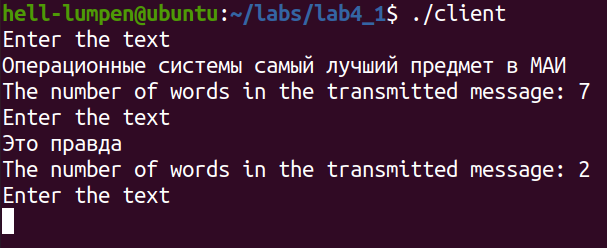
\includegraphics{4_1.png}}
\caption{Пример работы приложения.}
\label{1.png}
\end{figure}
\newpage

\subsection{Чат}
\subsubsection{Техническое задание}
Написать сетевое приложение --- чат. Оно должен делать следующее: 
\begin{enumerate}
	\item Пользователь через аргументы задаёт 2 параметра:
	\begin{itemize}
		\item -a IP\_адрес:порт (пример \texttt{-a 127.0.0.1:1024});
		\item -u имя\_пользователя (пример \texttt{-u Ali}).
	\end{itemize}
	\item Приложение по указанному порту отсылает вводимые пользователем сообщения и печатает принимые сообщения. Перед любым сообщением указывается логин пользователя (пример \texttt{Ali: Hello!}).
	\item Выход из приложения выполняется по вводу строки <<quit!>>.
	\item Общение происходит через протокол UDP. (SOCK\_DGRAM) 
\end{enumerate}

\subsubsection{Описание основного алгоритма}
Алгоритм парсит полученные через аргументы командной строки ip-адрес, порт и имя собеседника. Создается сокет и привязывается к заданному адресу. Создается структура c сетевым адресом посредством функции \verb|inet_pton|. Создается процесс-потомок. Процесс потомок занимается отправкой сообщений по заданному адресу. Процесс-родитель принимает сообщения и выводит их в консоль пользователю. 

Реализация алгоритмов представлена в разделе приложения \ref{code:lab4_2}.

\subsubsection{Руководство пользователя}
Пользователям необходимо набрать в консоли команду \verb|ifconfig|, чтобы узнать ip-адрес машины. Ввести этот адрес на другой машине через аргументы командной строки и через двоеточие написать порт. Портом может быть любая цифра, главное чтобы она была одинаковая у двух пользователей (для корректной работы рекомендуется использовать номер порта, чье значение больше 1024, т.к. порты до этого значения могут быть заняты системными приложениями). Для завершения чата нужно набрать команду \verb|quit!|.
\begin{figure}[h!]
\center{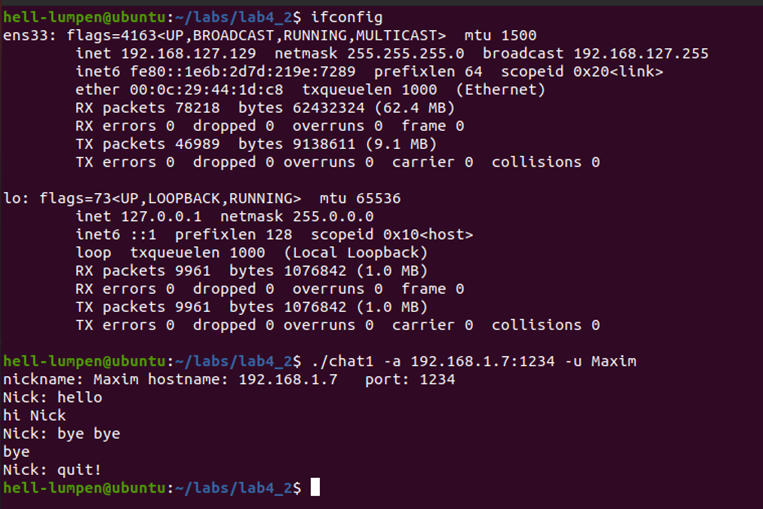
\includegraphics{4_2_1.png}}
\caption{Приложение - Чат. Клиент 1.}
\label{1.png}
\end{figure}

\begin{figure}[H]
\center{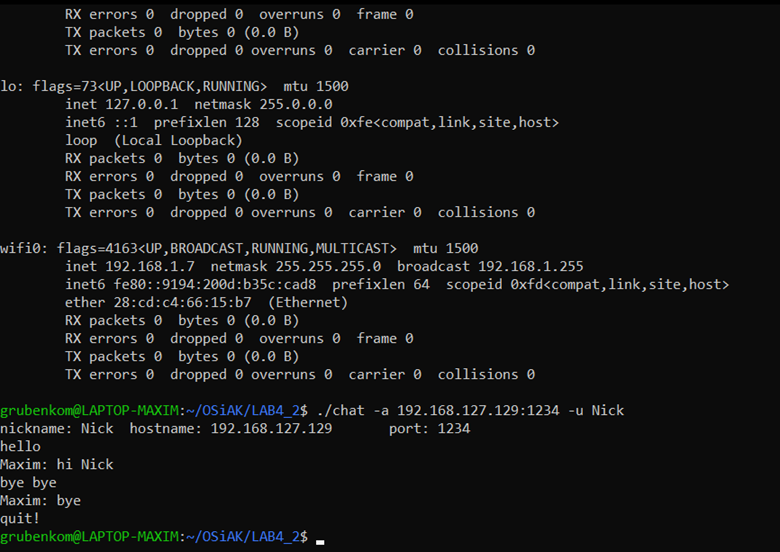
\includegraphics{4_2_2.png}}
\caption{Приложение - Чат. Клиент 2.}
\label{1.png}
\end{figure}

\newpage
\
\part{Индивидуальная часть}
%В каждом из подразделов нужно описать 

\section{Клиент-серверное ПО <<\SOFTWARE>>}

\subsection{Техническое задание}
Необходимо реализовать клиент-серверное приложение, имеющее следующую структуру:

\begin{figure}[h]
\center{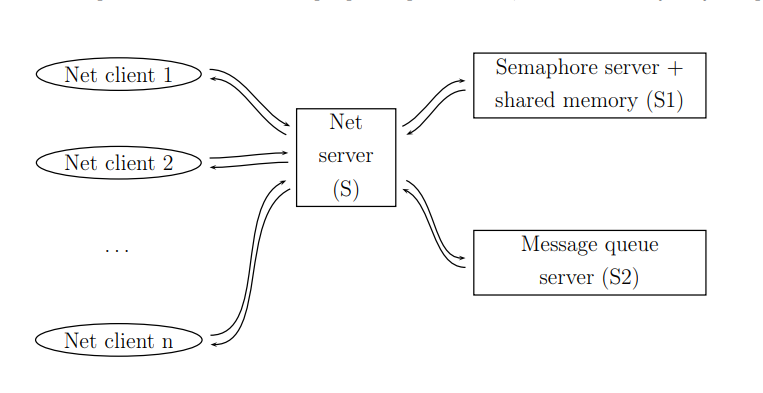
\includegraphics{struct.png}}
\caption{Структура программного комплекса.}
\label{1.png}
\end{figure}
 
Сетевой сервер принимает 2 типа запросов от клиентов: 
\begin{enumerate}
	\item решение задачи <<Частотный анализ встречающихся символов в файле. Построение гистограммы>>;
	\item решение задачи <<Калькулятор длинных чисел>>.
\end{enumerate}
Используя данные, передаваемые от клиента по первому типу запроса, сетевой сервер \textbf{S} формирует запрос к серверу \textbf{S2}, а по второму типу запроса --- к серверу \textbf{S1}. Серверы \textbf{S1} и \textbf{S2} формируют соответствующие задачам ответы, которые сервер \textbf{S} транслирует инициирующему клиенту. 

\subsection{Формулировка задачи 1}
Подсчёт частоты встречающихся букв в пересланных файлах. Файлы пересылаются по очереди, частоты пересчитываются от общей суммы файлов.

\subsection{Формулировка задачи 2}
Калькулятор длинных чисел. Поддерживаются операции сложения и вычитания.

\subsection{Протокол общения клиента и сервера \textbf{S}}
Сокет основан на протоколе TCP. Клиент отправляет строку с задачей, а сервер принимает ее и определяет тип задачи. По нему сервер \textbf{S} переадресовывает запрос к необходимому серверу \textbf{S1} или \textbf{S2}.

\subsection{Протокол общения серверов \textbf{S} и \textbf{S1}}
Сервер \textbf{S1} занимается обработкой запросов, связанных с арифметическими операциями с длинными числами. Сервер \textbf{S} отправляет полученную строку, если она подходит по типу решаемых задач. \textbf{S} кладет строку в разделяемую память, которую открыл сервер \textbf{S1}. Далее \textbf{S1} обрабатывает полученное из разделяемой памяти сообщение и загружает ответ в память в виде строки, которая содержит ответ на поставленную задачу, либо --- текст возникшей ошибки.

\subsection{Протокол общения серверов \textbf{S} и \textbf{S2}}
Сервер \textbf{S2} обрабатывает запросы типа 1 --- запрос на частотный анализ встречающихся символов в переданном файле. Сервер \textbf{S} добавляет в очередь строку, которая содержит имя файла. \textbf{S2} обрабатывает файл и создает новый файл, в котором содержится статистика по встречающимся символам. Имя этого файла сервер добавляет в очередь, откуда его считает сервер \textbf{S}. Файл получает клиент и с помощью специальной функции открывает и обрабатывает его для вывода информации в консоль пользователю.

\subsection{Структура приложения}

Главный сервер \textbf{S} создает сокет для обмена сообщениями с клиентом. Клиент также создает сокет и подключается к локальному адресу. 
Далее клиентская программа заходит в бесконечный цикл общения с главным сервером. У пользователя запрашивается номер запроса и сам запрос. На основе этих данных формируется сообщение, путем конкатенации символа, обозначающего тип задачи и C-style строки с самим запросом. Затем клиент отправляет это сообщение главному серверу \textbf{S}, где сервер читает первый символ принятой строки и определяет тип запроса и совершает переадресацию нужному серверу. Для первой задачи --- сервер на очереди сообщений (\textbf{S2}), для второй задачи --- сервер на разделяемой памяти и семафорах (\textbf{S1}). Главный сервер отправляет сообщения по протоколу, который реализует вспомогательный сервер, и ожидает ответа от него. Внутри каждого вспомогательного сервера реализованы специальные функции, которые обрабатывают входящие сообщения, формируют ответ и отправляют его главному серверу, который в свою очередь перенаправляет его клиенту, инициировавшему запрос.

Все функции, которые используются в главном сервере и клиенте, реализованы как <<обертки>>, для более удобной обработки ошибок. Их реализация содержится в файле \verb|wrappers.h|.

Функции, реализующие операции с длинными числами находятся в заголовочном файле \verb|bigint.h|.

Функции, проводящие анализ содержимого файла, находятся в заголовочном файле \verb|analyzer.h|.

\subsection{Основные алгоритмы}
Алгоритм анализа символов в файле реализуется с помощью функций:

1. \verb|char* analiz(char* pathname, std::map<char, size_t> &dict)|;

2. \verb|void count_symbols(std::map<char, size_t> &dict, std::string str)|;

3. \verb|void print_file_gistogram(char* pathname)|.

Первая функция открывает файл, название которого передал пользователь, читает его построчно, запуская для каждой прочитанной строки функцию \verb|count_symbols|. В параметры передается считанная строка и структура \verb|std::map|, которая хранит статистику всех файлов, которые передал пользователь. Возвращает C-style строку с именем файла в котором содержится статистика или текстовое описание ошибки, возникшей во время работы программы.

Вторая функция проходит с помощью цикла по всей строке, занося каждый новый символ в структуру, и, увеличивая счетчик тому символу, что уже встречался.

Третья функция необходима клиенту для того, чтобы представить содержимое файла на консоли у пользователя в удобном виде. Она считывает построчно файл, в котором содержится информация в формате:
<<символ\_пробел\_количество>>.

Алгоритм суммы и вычитания больших чисел реализуется с помощью функций:

1. \verb|_to_number(char character)|

Переводит символ числа в само число типа \verb|int| путем вычитания ascii кода символа <<0>>.

2. \verb|_to_char(int number)|

Данная функция проводит обратное действие первой функции. К числу прибавляется ascii код символа <<0>>.

3. \verb|_remove_leading_zeros(string &result)|

Функция удаляет символ <<0>> в строковом представлении числа, который мог там появиться вследствие вычислений.

Функция \verb|string add(int base, string num1, string num2)| складывает два числа, которые представлены в строковом формате. Для начала производится перезапись числа в обратном порядке, чтобы можно было производить операции с числом как это делает человек. С помощью вышеописанных функций от каждого i-символа строки выделяется число, с которым производится простая арифметическая операция --- сложение двух целочисленных значений. В конце полученное число переводится в символ числа и сформированная строка вновь перезаписывается в обратном порядке, чтобы получить корректный вид строкового представления результата. В завершении удаляются ведущие нули, если они появились в процессе вычисления.

Функция вычитания \verb|string sub(int base, string num1, string num2)| устроена аналогично сложению. Функция работает с числами, также как это привычно делал бы человек, вычисляя разность <<столбиком>>. 

В файле \verb|wrappers.h| кроме оберток реализованы функции для работы с семафорами, отправки и приема сообщений для сервера основанному на разделяемой памяти.

Функция \verb|void change_semafores(int semID, SEM_OP type)| проводит операции с массивом семафоров с дескриптором \verb|semID|. Операция определяется по типам. Перечисление \verb|enum SEM_OP| содержит все возможные операции для семафоров.

Функции \verb|void send_msg(char *shm_ptr, char *msg, int semid, bool is_server)| и \verb|void recv_msg(char *shm_ptr, char *msg, int semid, bool is_server)| занимаются отправкой и приемом сообщений соответственно. Производятся необходимые действия с семафорами для корректного доступа к памяти и копирование содержимого из буфера в сегмент разделяемой памяти или из памяти --- в буфер.

Также в файле \verb|wrappers.h| определены константы \verb|PORT| и \verb|MSG_SIZE|. Первая отвечает за номер порта по которому подключаются главный сервер и клиент, вторая --- за размер сообщений, которые передаются между клиентом и серверами.

Реализация алгоритмов представлена в разделе приложения \ref{code:soft}.

\subsection{Руководство пользователя}

\begin{figure}[h]
\center{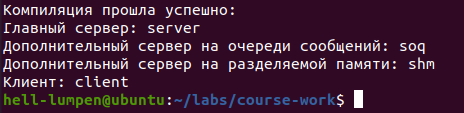
\includegraphics{compile.png}}
\caption{Успешный запуск приложения после компиляции исходных файлов.}
\label{1.png}
\end{figure}

Запустить программу можно с помощью специального скрипта \verb|run_servers|. Допускается запуск с ключом \verb|-c|. В этом случае скрипт удалит предыдущие исполняемые файлы и снова компилирует весь проект и запускает все сервера и одного клиента, если компиляция пройдет успешно. Чтобы запустить приложение без компиляции необходимо прописать в терминале команду \verb|./run_servers| без аргументов. Скрипт запустит одного клиента и три сервера. Чтобы запустить еще одного клиента необходимо открыть дополнительное окно терминала и ввести команду \verb|./client|.

Пользователя приветствует главное меню с выбором типа задачи.

\begin{figure}[h]
\center{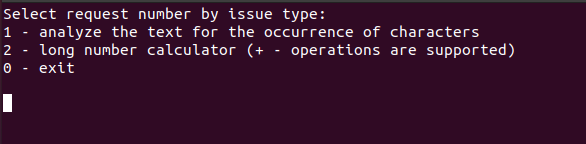
\includegraphics{interface.png}}
\caption{Главное меню приложения.}
\label{1.png}
\end{figure}

Доступны два типа задачи. Для выбора необходимого нужно в консоли набрать цифру, соответствующую подходящему, для пользователя, типу задачи. Для выхода из приложение необходимо ввести <<0>>.

\begin{figure}[h]
\center{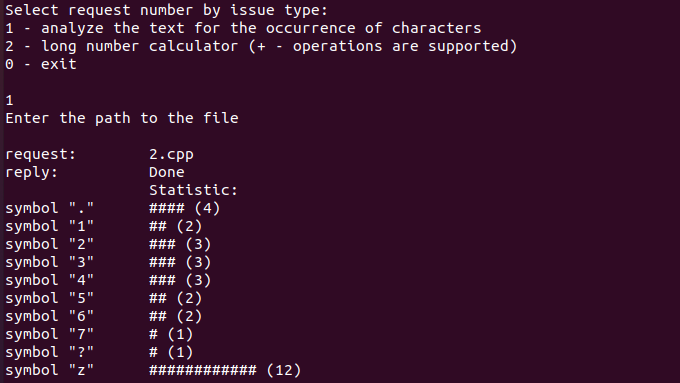
\includegraphics{task1.png}}
\caption{Пример решения задачи первого типа.}
\label{1.png}
\end{figure}

При выборе задачи первого типа, программа запросит имя файла. Программа проведет анализ входного файла. Если передать еще один файл, то гистограмма будет пересчитана с учетом предыдущих запросов.

\begin{figure}[H]
\center{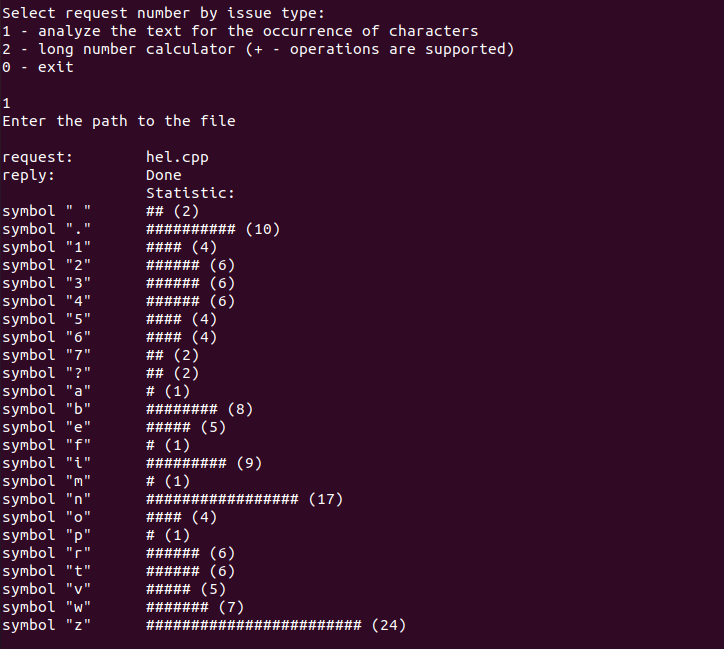
\includegraphics{task1.1.png}}
\caption{Пересчет статистики при передаче еще одного файла.}
\label{1.png}
\end{figure}

Если файл не существует или возникнет какая-то ошибка при подсчете статистики пользователь будет об этом уведомлен.

\begin{figure}[H]
\center{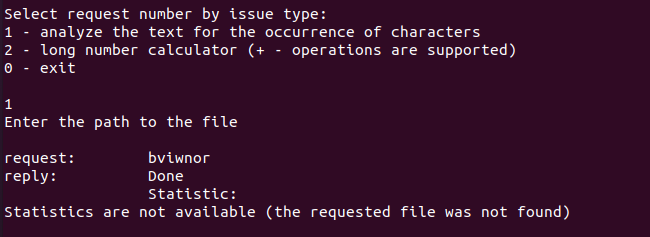
\includegraphics{task1.2.png}}
\caption{Аномальные входные данные.}
\label{1.png}
\end{figure}

При выборе задачи второго типа программа запросит арифметическое выражение. Важно, чтобы числа и знак не были разделены какими-либо символами.

\begin{figure}[H]
\center{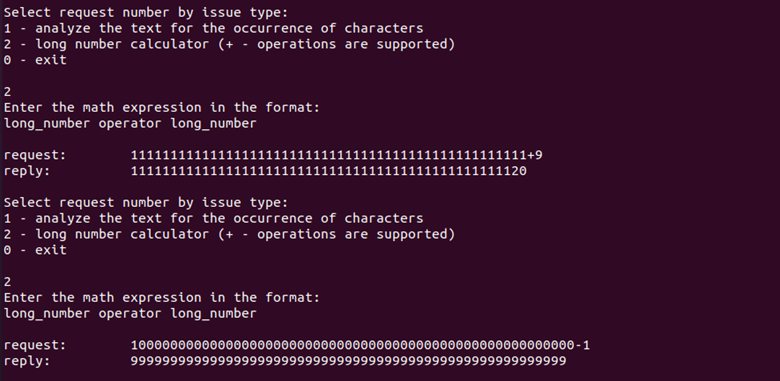
\includegraphics{task2.png}}
\caption{Корректная работа приложения.}
\label{1.png}
\end{figure}

Если пользователь передаст некорректное выражение, он получит сообщение об ошибке.

\begin{figure}[H]
\center{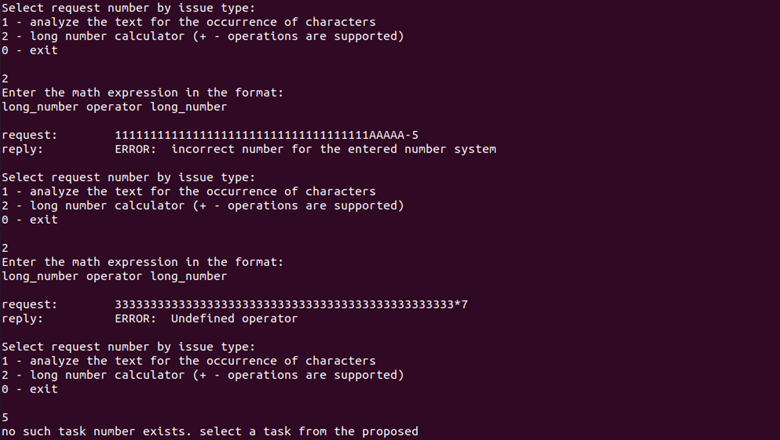
\includegraphics{task2.1.png}}
\caption{Аномальные входные данные.}
\label{1.png}
\end{figure}

\newpage

\section{Список использованных источников}
Эндрю С. Таненбаум, Т. Остин. Архитектура компьютера (Structured Computer Organization). --- 5-е издание. --- СПб : Питер, 2010.

Чан Т. Системное программирование на C++ для Unix. : BHV, 1997.

\href{https://www.opennet.ru/man.shtml}{https://www.opennet.ru/man.shtml}

\href{https://intuit.ru/academies/companiesn/41/info}{Курс <<Академия Intel: Основы операционных систем. Практикум>>. НОУ ИНТУИТ}

\href{https://habr.com/ru/post/330676/}{Client-Server step by step. habr.com}

\href{https://habr.com/ru/post/122108/}{Знакомство с межпроцессным взаимодействием на Linux. habr.com}

\newpage

\section{Приложение}

\subsection{Калькулятор}\label{code:lab1_1}
\centerline{\textbf{Файл \texttt{lab1\_1\_main.cpp}}}

\inputminted{octave}{lab11main.cpp}

\centerline{\textbf{Файл \texttt{lab1\_1\_calc.cpp}}}

\inputminted{octave}{lab11calc.cpp}

\subsection{Порождение процессов}\label{code:lab1_2}
\centerline{\textbf{Файл \texttt{lab1\_2.cpp}}}

\inputminted{octave}{lab12.cpp}

\subsection{Реализация ls}\label{code:lab2_1}
\centerline{\textbf{Файл \texttt{lab2\_1.cpp}}}

\inputminted{octave}{lab21.cpp}

\subsection{Реализация ls без папок}\label{code:lab2_2}
\centerline{\textbf{Файл \texttt{lab2\_2.cpp}}}

\inputminted{octave}{lab22.cpp}

\subsection{Жесткая ссылка}\label{code:lab2_3}
\centerline{\textbf{Файл \texttt{lab2\_3.cpp}}}

\inputminted{octave}{lab23.cpp}

\subsection{Символическая ссылка}\label{code:lab2_4}
\centerline{\textbf{Файл \texttt{lab2\_4.cpp}}}

\inputminted{octave}{lab24.cpp}

\subsection{Сортировка файлов}\label{code:lab2_5}
\centerline{\textbf{Файл \texttt{lab2\_5.cpp}}}

\inputminted{octave}{lab25.cpp}

\subsection{Клиент-сервер на очереди сообщений}\label{code:lab3_1}
\centerline{\textbf{Файл \texttt{server.cpp}}}

\inputminted{octave}{server31.cpp}

\centerline{\textbf{Файл \texttt{client.cpp}}}

\inputminted{octave}{client31.cpp}

\subsection{Клиент-сервер семафорах и разделяемой памяти}\label{code:lab3_2}
\centerline{\textbf{Файл \texttt{server.cpp}}}

\inputminted{octave}{server32.cpp}

\centerline{\textbf{Файл \texttt{client.cpp}}}

\inputminted{octave}{client32.cpp}

\subsection{Клиент-сервер на протоколе TCP}\label{code:lab4_1}
\centerline{\textbf{Файл \texttt{server.cpp}}}

\inputminted{octave}{server41.cpp}

\centerline{\textbf{Файл \texttt{client.cpp}}}

\inputminted{octave}{client41.cpp}

\centerline{\textbf{Файл \texttt{wrappers.h}}}

\inputminted{octave}{wrappers41.h}

\subsection{Клиент-сервер на протоколе UDP}\label{code:lab4_2}
\centerline{\textbf{Файл \texttt{chat.cpp}}}

\inputminted{octave}{chat.cpp}

\subsection{Клиент-серверное приложение для анализа файлов и калькулятор длинных чисел}\label{code:soft}

\centerline{\textbf{Файл \texttt{run\_servers}}}

\begin{verbatim}
#!/bin/bash

if [[ "$1" == -c ]]
then

rm server
rm client
rm soq
rm shm

clear

g++ main_server.cpp -o server
g++ client.cpp -o client
g++ server_on_queue.cpp -o soq
g++ server_on_shared_memory.cpp -o shm

if [ -e server ] && [ -e client ] && [ -e soq ] && [ -e shm ]
then

echo "Компиляция прошла успешно:"
echo "Главный сервер: server"
echo "Дополнительный сервер на очереди сообщений: soq"
echo "Дополнительный сервер на разделяемой памяти: shm"
echo "Клиент: client"

else

echo "Ошибка компиляции"

fi

fi

if [ -e server ] && [ -e client ] && [ -e soq ] && [ -e shm ]
then

gnome-terminal --tab -- "./soq"
gnome-terminal --tab -- "./shm"
gnome-terminal --tab -- "./server"
gnome-terminal --tab -- "./client"

else

echo "Ошибка. Запуск невозможен"

fi
\end{verbatim}

\centerline{\textbf{Файл \texttt{main\_server.cpp}}}

\inputminted{octave}{mainserver.cpp}

\centerline{\textbf{Файл \texttt{server\_on\_queue.cpp}}}

\inputminted{octave}{serveronqueue.cpp}

\centerline{\textbf{Файл \texttt{server\_shared\_memory.cpp}}}

\inputminted{octave}{serveronsharedmemory.cpp}

\centerline{\textbf{Файл \texttt{wrappers.h}}}

\inputminted{octave}{wrappers.h}

\centerline{\textbf{Файл \texttt{analyzer.h}}}

\inputminted{octave}{analyzer.h}

\centerline{\textbf{Файл \texttt{bigint.h}}}

\inputminted{octave}{bigint.h}

\end{document}
